\section{Feedback and interaction methods for the user}

Cognitive load plays an important role if skill acquisition is a major factor. In slacklining the user has to focus on multiple things simultaneously that increases the mental pressure. The system has to be aware of this to restrict it in the right way, which results in useful feedback for the user. Another important fact is that repetitive exercises can lead to a boring and demotivating user experience. For that reason several methods, systems and game approaches can be used as an inspiration to build a system with a motivating and joyful environment. At last the integration and visualisation of feedback and interaction methods should be well thought out. Several techniques have been elaborated on how to provide this appropriately.

\subsection{Restricting cognitive load}

As a baseline Paas et al. \cite{Paas2003-xt} describes that the acquisition of new skills is in conjunction with cognitive load. By adjusting this the learning effect can be easened or hardened. Three types of cognitive loads exists that handle the working memory of a person regarding the learning process. Intrinsic load is the inherent complexity that is caused by the topic itself. It is also important in which manner information is given to the user. If this is unnecessary, repetitive or interferes him it is called an extraneous cognitive load and increases the burden of the user. The last type is germane cognitive load, which describes also how information is given to the user but by supporting the him in that way. This is brought by activating and automating already existing patterns or generating new ones in the working memory to enhance a learning process. Regarding this several application have been evaluated that are also relevant to the slacklining supporting system.

Van der Spek \cite{Van_der_Spek2010-fe} evaluated how to deal with the right complexity in serious games. He describes in his mental model construction (Figure \ref{fig:mentalModelConstruction}) that interference can be avoided by information regulation and focus attention. Improving is encouraged by predictability and reflection of the tasks. The attention of the user should be focused to relevant material by regulating the information given to him. Since a serious game like approach should be developed this is an important reference for building an effective learning process to the user.

\begin{figure}[htb]
	\centering
	\begin{minipage}[t]{0.8\linewidth}
		\centering
		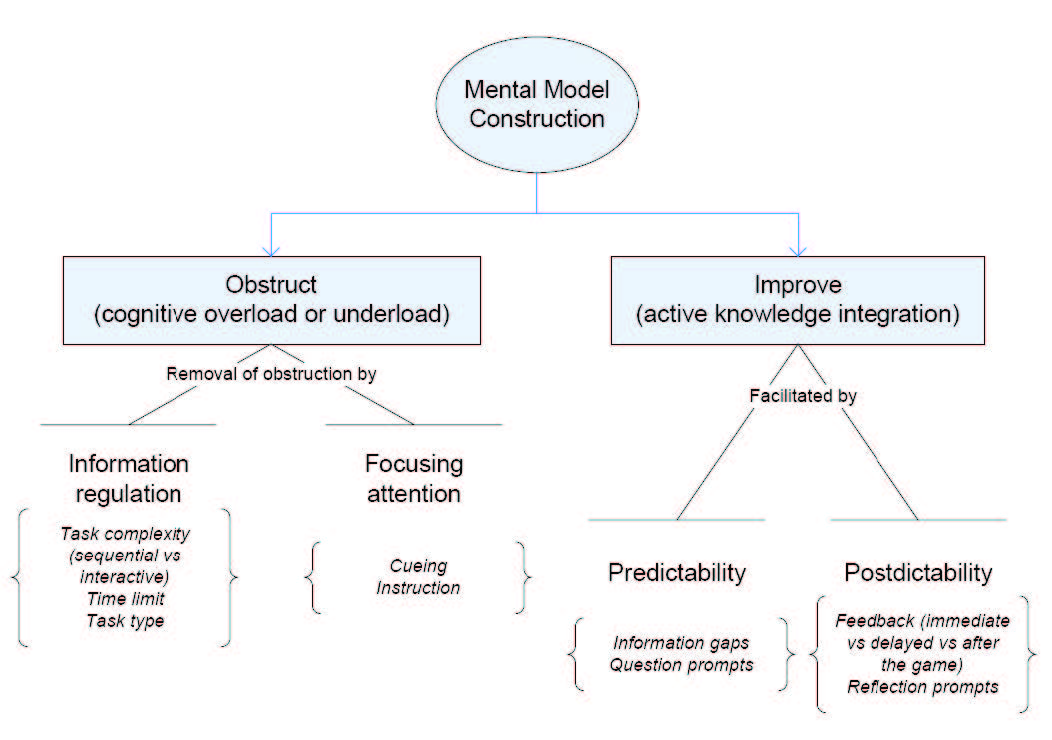
\includegraphics[width=1\linewidth]{Pictures/mentalModelConstruction}
		\caption{Guideline for enhancing the cognitive load \cite{Van_der_Spek2010-fe}}
		\label{fig:mentalModelConstruction}
	\end{minipage}
\end{figure}

Pisan et al. \cite{Pisan2013-sf} evaluates the user risk of falling with cognitive loading exercises. They executed two stroop tests, where the participant had to name the correct color of the word. High and low cognitive load can be measured by differentiating the meaning and color of a word. In the next challenge she has to answer different maths problems provided by the system. The results show that the reaction time due to cognitive load is much larger with users that have a higher risk of falling than for users that have a lower risk. This could be explainable due to the fact that user with higher falling risk are not that good in terms of switching the cognitive focus from the balancing action into other actions. Training on a slackline provides cognitive load to the user because of several simultaneously things she has to be aware of. Hence feedback given by the system on how to behave in a situation should be provided in an appropriate manner to support and restrict the cognitive capability.

\subsection{Motivating factors for skill acquisition}

Several rehabilitation and sport training programs can be elaborated because the skill acquisition in slacklining resemble with them. It is a process of repetitive exercise execution. For mastering new skills and extend himself a user must have the willingness and commitment for practicing, which can be described as motivation. The self-determination theory by Ryan et al. \cite{Ryan2000-gi} \cite{Ryan2000-jn} describes several types of motivational factors. First the intrinsic motivation, which is caused by interest to an action and satisfies the own psychological needs for self-determined behavior. This is the fundamental stimulus for high valuable learning and practicing. Second the extrinsic motivation that is performing an activity because of an external output. The user can hereby feel externally propelled due to compliance with external regulations or she can be self-endorsed due to willingness and acceptance by the value of the practice. 

Johnson et al. \cite{Johnson1998-hb} stated regarding rehabilitation training that if exercises and the user himself provide negative factors like boredom, repetition or long execution time it results in a discouragement. Enhancing the interaction with this trainings can lead to effective training. 
Pisan et al. \cite{Pisan2013-sf} says that video games can help to motivate the patients through their physical training. The participants in his user tests found the games that he developed engaging. They preferred doing the exercises with the system.

Several researchers involved the motivational aspect of video games in their system. Ustinova et al. \cite{Ustinova2014-ml} developed four custom virtual video games to elaborate the efficacy for postural deficits. First a virtual teacher where the subject has to copy its movements strictly. Second a virtual challenger that is divided into a skateboard, courtyard and an octopus game with specific exercises in which the movements of the user are more flexible. Successfully completed performance will be rewarded with a number of points. Overall the user were strongly satisfied with the gaming part of the therapy and moderate with the virtual teacher part.

Freitas et al. \cite{Freitas2012-ae} focused on user centred development of a physiotherapeutic game that supports motor rehabilitation exercises. A plane represented the user and she has to fly through rings in the air and avoid obstacles. The patients were strongly satisfied with the game. An important factor here is the good user interface that affects the user motivation, visually presented scenario and playing technique in a positive way.

Estepa et al. \cite{Estepa2016-oj} evaluates three developed exergames involving different psychophysical rehabilitation exercises. A virtual avatar represents the patient and orders are giving via an auditive or visual stimuli. The first two games are a series of coming balls placed at desired angles that the patient has to avoid with her trunk or, in the second game, with her feet. In the third exercise she has to step forward to a colored line between starting and goal position. All games were easy to understand and provide necessary feedback. The patients had a considerable interest to use the system.

Kajastila and Hämäläinen \cite{Kajastila2014-ug} encourages monotonous parts of climbing training by adding goals and supporting the social collaboration of the participants. Hence they are making it overall more enjoyable. Six prototypes were developed. Prototypes that rely more on a training part are an easy route builder, automatic route generator and instant video feedback. For the user those were the most useful ones. The exercises that consists of a more playful part, such as a chasing animated saw that the climber has to avoid, shifted the focus away from the training part. 

With this in mind an useful training device should be considered that includes an enjoyable virtual environment. A good balance between these both is the key for successful and motivating skill acquisition.

\subsection{Approaches and techniques for providing feedback}

Several  useful technological advances like video feedback, virtual environments and auditive information can be applied for providing feedback in sport activities. Liebermann et al. \cite{Liebermann2002-zr} evaluated those regarding their field of application. With video information costs are relatively low, it is easy accessible, and portable. It can be repetitively replayed in real-time or superposition of two footages. Training in 3D virtual environments can help to improve or to familiarize with a real world skill acquisition. This is because the user can pre-practice a skill in simulated unknown conditions like pilots in a simulated airplane. Providing appropriate auditive information can also have a relatively high impact on performance enhancement. Also the Microsoft HCI-Guidelines state that implementing audio  is a good way if the user need to be notified adn to indicate states of changing behaviour \cite{MicrosoftHIG2014-mh}. For example in balance training a warning signal can indicate that the current pose is not the desired one. If the user corrects his posture in the right way, the signal should then transform into an more comfortable signal. All of these allow qualitative and meaningful feedback in their application context. The performer can review the execution, pre practice in a virtual environment, or be supported with audio warning signals. Therefore she can discover failure in her performance.

Feedback has to be provided in an appropriate manner for improving new motor skill acquisition. Especially for starting to learn a new technique it is important to have immediate feedback sources on which the user can rely on \cite{Hodges2002-gb} \cite{Winstein1990-to}. Therefore it should be easy to understand for enhancing the learning process. 

Hämäläinen \cite{Hmlinen2004-ai} developed applications for a camera output in front of the user. An automated motion controlled approach starts and stops the recording if the motion exceeds a certain threshold. Second a speech and last a gesture control prototype that consists of four commands to record, play, stop and delay the recording. The user test ranked the automatisation the worst because it reacted to unintentional motions, which ends in unwanted command recognition. The speech system ranked the best but only worked well if the participant speaks near the microphone. Some participants mentioned that the gesture approach were more intuitive and natural, which could be a good compromise out of the three approaches.

Holsti et al. \cite{Holsti2013-kn} investigated delayed video feedback and a platform jumping game in trampoline sport. The former records the performance execution and shows it repetitive to the user. In the second the player has to jump back- and forwards on virtual platforms. They tested it with athletes and beginner. The delayed video feedback was ranked useful for nearly all athletes. Overall the platform jumping game was ranked the best.

Kajastila and Hämäläinen \cite{Kajastila2014-ug} project graphics onto an artificial climbing wall. A feasibility study showed that the graphic information is best located near holds where the focus of the climber goes naturally. This can be adapted to the slacklining system since the focus is usually set onto a specific point in front of the user. It would be therefore useful to provide information in the peripheral view. Next to other prototypes he has implemented an instant delayed video feedback. This is rated as one of the most useful ones because the user can immediately analyse her performance. Also a gaming approach is developed as an animated saw that chases the climber and which she has to avoid. User testing resulted that it moves the focus away from the training, but it could be an enjoyable alternative to kids for getting them used to the sport. 

Based on the results of the last paper Kajastila et al. \cite{Kajastila2016-ot} developed two games and a route creation application. User emphasize the versatility and excitement of the games. They also forget the fear of heights due to time limits and forcing them to focus and achieve a goal. User stated that playing and spectating is also more fun due to implemented sound and visual effects.

A well defined interaction mechanism and a good looking environment can help to create an effective system and motivate the user for training purposes. A delayed video feedback is a good approach to learn new skills. Combining this with a gaming approach can simultaneously lead to a joyful experience with training aspects. Also adding audio signals can further improve this experience for the user as well as for spectators.

\subsection{User interface}

Important feedback information during the exercise should be placed surrounding the focus point in the peripheral view of the user. Directing the user for correcting her movement can be done in several ways. Basic information about the execution should be given prior to the user for exercise preparation. Surrounding objects can be displayed as arrows, flashing notifications or weighting scale like seen by Garrido Navarro et al. \cite{Garrido2013-zs} in Figure \ref{fig:informationUISurroundingObjects}. Additional informations like current exercise and the state can be displayed outside of the focus space. But they should be designed to not distract the user. If they do so it should be able to just show the feedback visualisations. A feedback summary after the execution can give an useful resume about the exercise as an reflection like in Figure \ref{fig:informationUIFeedbackSummary}.

\begin{figure}[htb]
	\centering
	\begin{minipage}[t]{0.49\linewidth}
		\centering
		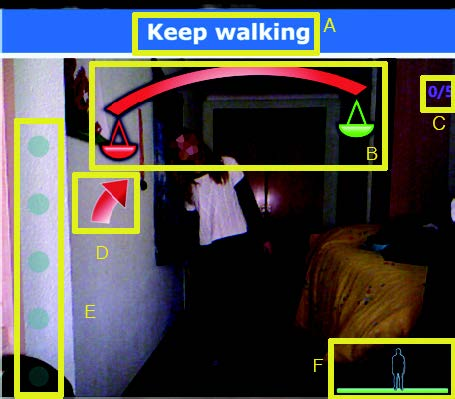
\includegraphics[width=1\linewidth]{Pictures/informationUISurroundingObjects}
		\caption{Surrounding objects in the UI \cite{Garrido2013-zs}}
		\label{fig:informationUISurroundingObjects}
	\end{minipage}
	\hfill
	\begin{minipage}[t]{0.49\linewidth}
		\centering
		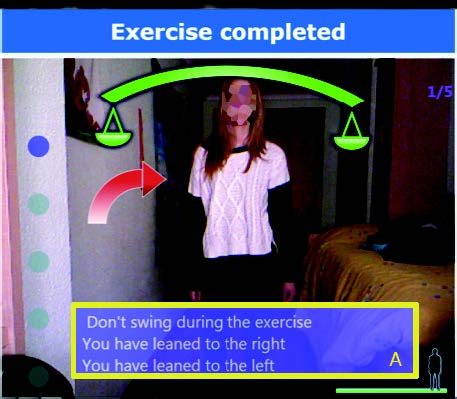
\includegraphics[width=1\linewidth]{Pictures/informationUIFeedbackSummary}
		\caption{Completed exercise feedback summary \cite{Garrido2013-zs}}
		\label{fig:informationUIFeedbackSummary}
	\end{minipage}
\end{figure}

Another method is to show the user itself or an avatar that demonstrates the correct performance of the current exercises like in Figure \ref{fig:avatar3DModel} and \ref{fig:avatarUser}. Holsti et al. \cite{Holsti2013-kn} implemented such a user integration and in user testing they endorse to see themself performing in real time.

\begin{figure}[htb]
	\centering
	\begin{minipage}[t]{0.49\linewidth}
		\centering
		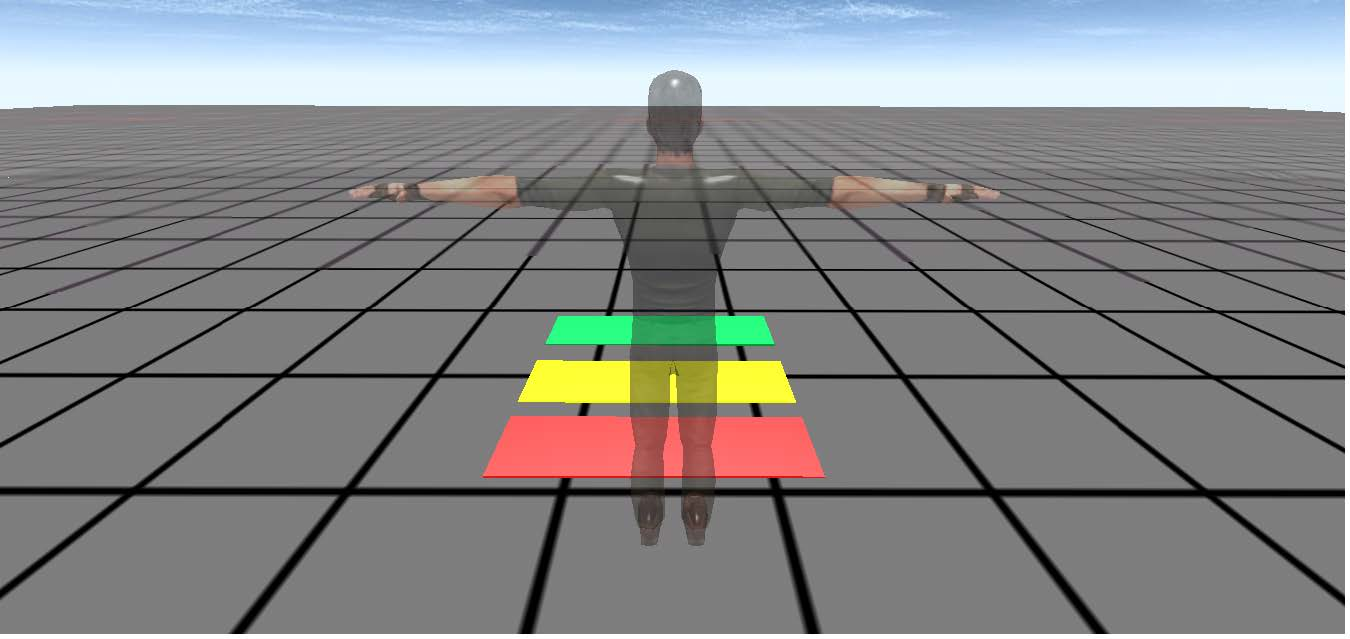
\includegraphics[width=1\linewidth]{Pictures/avatar3DModel}
		\caption{3D Model as avatar \cite{Estepa2016-oj}}
		\label{fig:avatar3DModel}
	\end{minipage}
	\hfill
	\begin{minipage}[t]{0.49\linewidth}
		\centering
		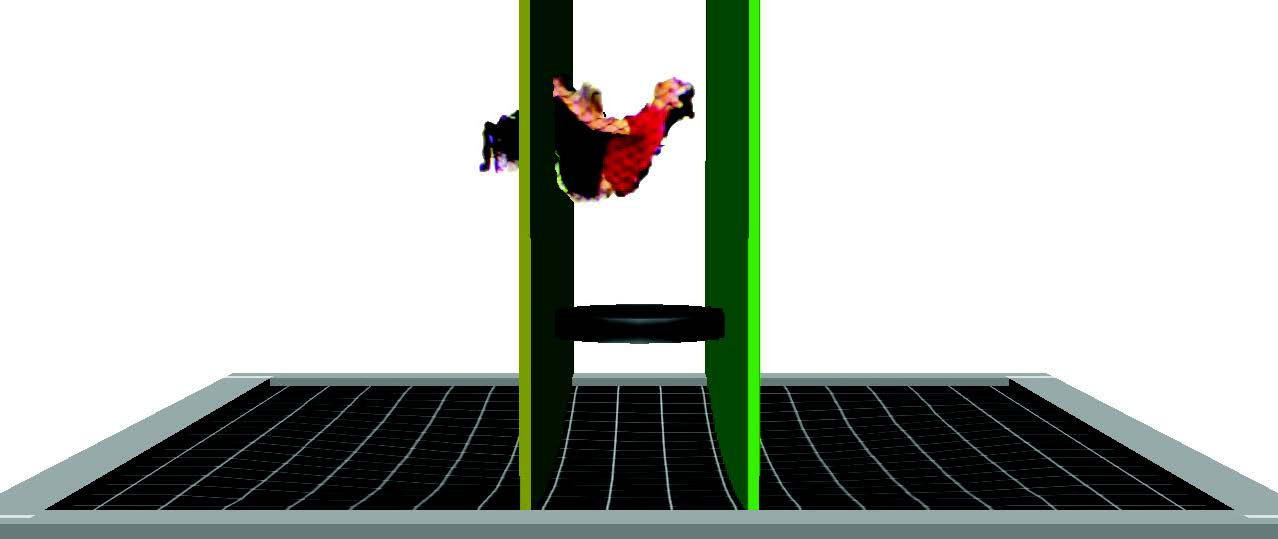
\includegraphics[width=1\linewidth]{Pictures/avatarUser}
		\caption{Rail-time user representation \cite{Holsti2013-kn}}
		\label{fig:avatarUser}
	\end{minipage}
\end{figure}

The task about the execution has to be clarified. Chang et al. \cite{Chang2012-hz} provides real time feedback on the performance quality due to a visualised path. If the performance is correct the path will turn green. But if she moves outside the range the path turns red and an arrows guides him into the correct position. Instructions and highlighting objects can help to complete an exercise successfully (Figure \ref{fig:gameInstruction} and \ref{fig:gameHighlighting}). If she performs something wrong during the performance e.g. in the slacklining case corresponding body parts could be highlighted.

\begin{figure}[htb]
	\centering
	\begin{minipage}[t]{0.49\linewidth}
		\centering
		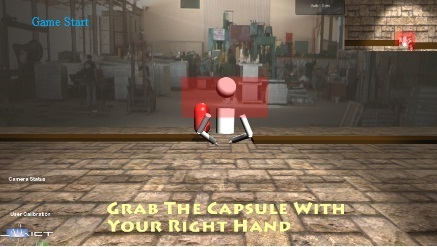
\includegraphics[width=1\linewidth]{Pictures/gameInstruction}
		\caption{Instruction to the game \cite{Chang2012-hz}}
		\label{fig:gameInstruction}
	\end{minipage}
	\hfill
	\begin{minipage}[t]{0.49\linewidth}
		\centering
		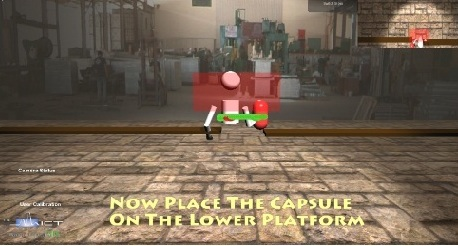
\includegraphics[width=1\linewidth]{Pictures/gameHighlighting}
		\caption{Green indicator for correct performance \cite{Chang2012-hz}}
		\label{fig:gameHighlighting}
	\end{minipage}
\end{figure}

Microsoft itself offers human interface guidelines for the Kinect v2 \cite{MicrosoftHIG2014-mh}. In this document is describes how to design and develop for the user. It provides a quick introduction into the Kinect itself, design principles for interactions regarding gesture and voice, and how to visualize appropriate feedback. Also which interactions should be used for a specific action. Overall design principles are that the application should be context-aware, make the user confident, choosing the right input method and to conduct user tests. A gesture that relies on the real world can help the user to be more familiar with the product, than learning unknown gestures (Figure \ref{fig:hciGuidelinesDynamicGesture}).

\begin{figure}[htb]
	\centering
	\begin{minipage}[t]{1\linewidth}
		\centering
		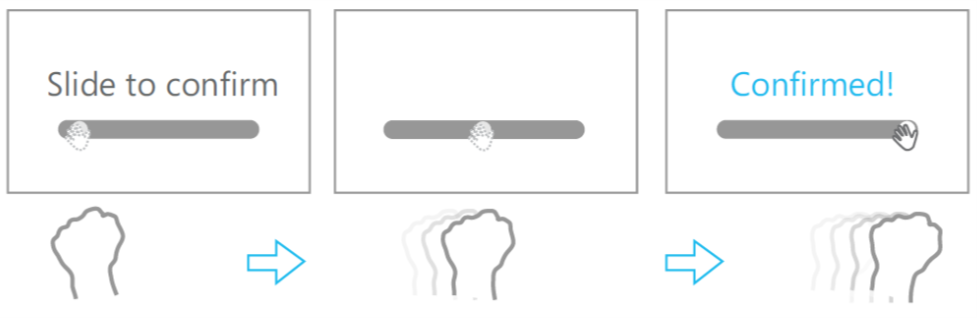
\includegraphics[width=0.5\linewidth]{Pictures/hciGuidelinesDynamicGesture}
		\caption{Slider as dynamic gesture \cite{MicrosoftHIG2014-mh}}
		\label{fig:hciGuidelinesDynamicGesture}
	\end{minipage}
\end{figure}

Teaching gestures is a core functionality in the slacklining assistance system. The HCI-Guidelines state that new gestures should be teached with a quick tutorial. Further a visual hint, animation, or notification can also help for first the engagement (Figure \ref{fig:hciGuidelinesTeachingMethods}).

\begin{figure}[htb]
	\centering
	\begin{minipage}[t]{1\linewidth}
		\centering
		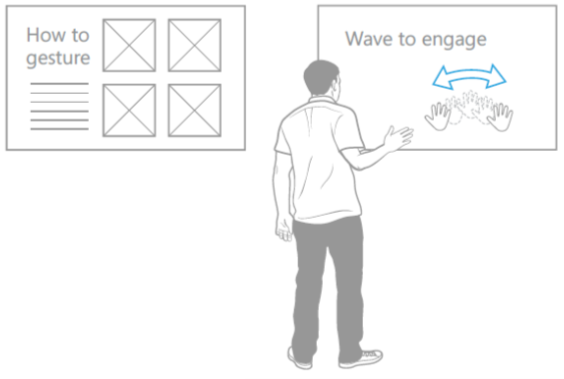
\includegraphics[width=0.4\linewidth]{Pictures/hciGuidelinesTeachingMethods}
		\caption{Teaching new gestures \cite{MicrosoftHIG2014-mh}}
		\label{fig:hciGuidelinesTeachingMethods}
	\end{minipage}
\end{figure}

Appropriate feedback should visualise if the sensor is ready, the user is visible to the Kinect, she is engaging right now, etc. For example if the user can control something with his hand can be visualised in form of a cursor and the state of a UI control element should also be clear (Figure \ref{fig:hciGuidelinesFeedback}).

\begin{figure}[htb]
	\centering
	\begin{minipage}[t]{0.45\linewidth}
		\centering
		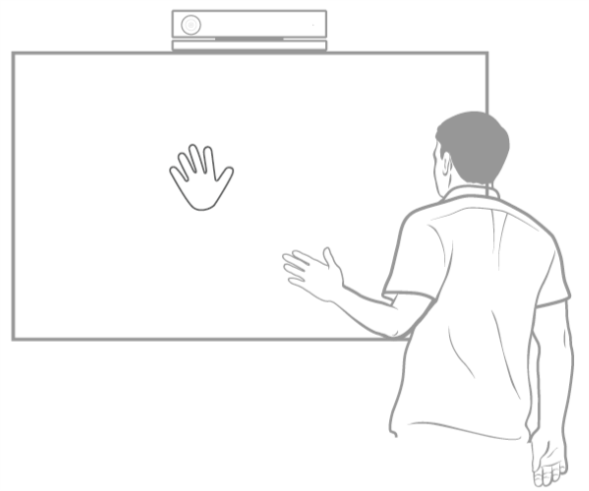
\includegraphics[width=0.5\linewidth]{Pictures/hciGuidelinesFeedbackCursor}
		\subcaption{Hand cursor}
		\label{fig:hciGuidelinesFeedbackCursor}
	\end{minipage}
	\hfill
	\begin{minipage}[t]{0.45\linewidth}
		\centering
		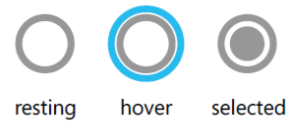
\includegraphics[width=0.5\linewidth]{Pictures/hciGuidelinesFeedbackControl}
		\subcaption{UI controls}
		\label{fig:hciGuidelinesFeedbackControl}
	\end{minipage}
	\caption{Feedback methods \cite{MicrosoftHIG2014-mh}}
	\label{fig:hciGuidelinesFeedback}
\end{figure}

The most important part is the progress indicator described in this guideline. It says that an idicator should be given if the user has to hold a position, as well as the frequency of gesture repetition. Clear and prominent visuals should be used to show the entire progression (Figure \ref{fig:hciGuidelinesProgressIndicator}). If a user should copy a specific movement an avatar or animation can be shown, before or during the movement.

\begin{figure}[htb]
	\centering
	\begin{minipage}[t]{1\linewidth}
		\centering
		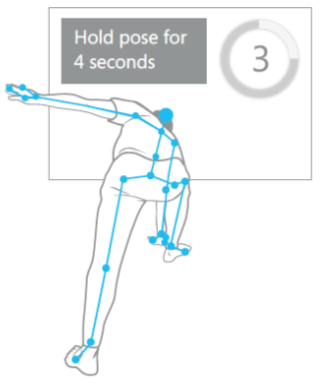
\includegraphics[width=0.3\linewidth]{Pictures/hciGuidelinesProgressIndicator}
		\caption{Repetition and time length indicators}
		\label{fig:hciGuidelinesProgressIndicator}
	\end{minipage}
\end{figure}

%Kann evtl nicht genutzt werden
%Displaying an avatar can be further implemented by a conjunction or overlapping with an instructor on the screen \textbf{(Figure 8)}. With this she can see wrong performance execution in real time. After the exercise she should be able to review her performance. At the same time the system has to be aware of not distracting the user too much during the performance. 